\chapter{Testing}
\label{ch:testing}
\section{Introduction}
Goals
\newpage

\begin{landscape}
	\section{Requirements Testing}
	\subsection{Functional Requirements}
	\begin{tabularx}{\hsize}{lXXXr}
		\toprule
		ID & Name & Expected Output & Evidence & Success? \\
		\midrule
		F1 & User Interaction 
		& A page should display to allow the user to interact with the bot
		& 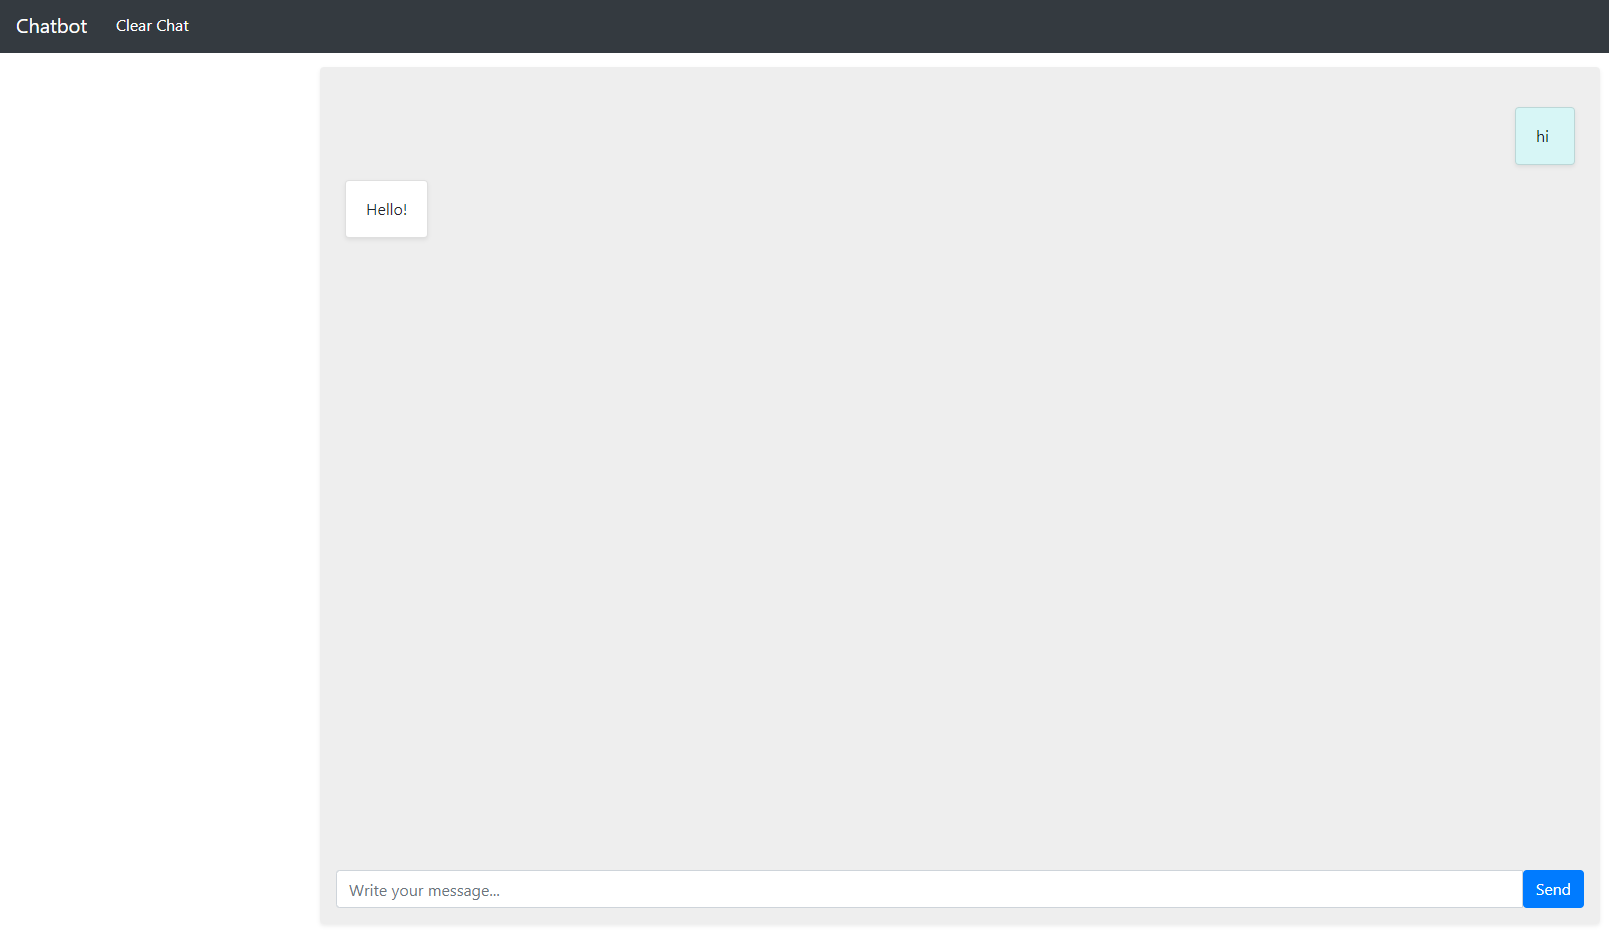
\includegraphics[width=8cm, valign=m]{tests/f1} & Yes \\
		\midrule
		F2 & Browser Access
		& The user should be able to access the system via a browser
		& 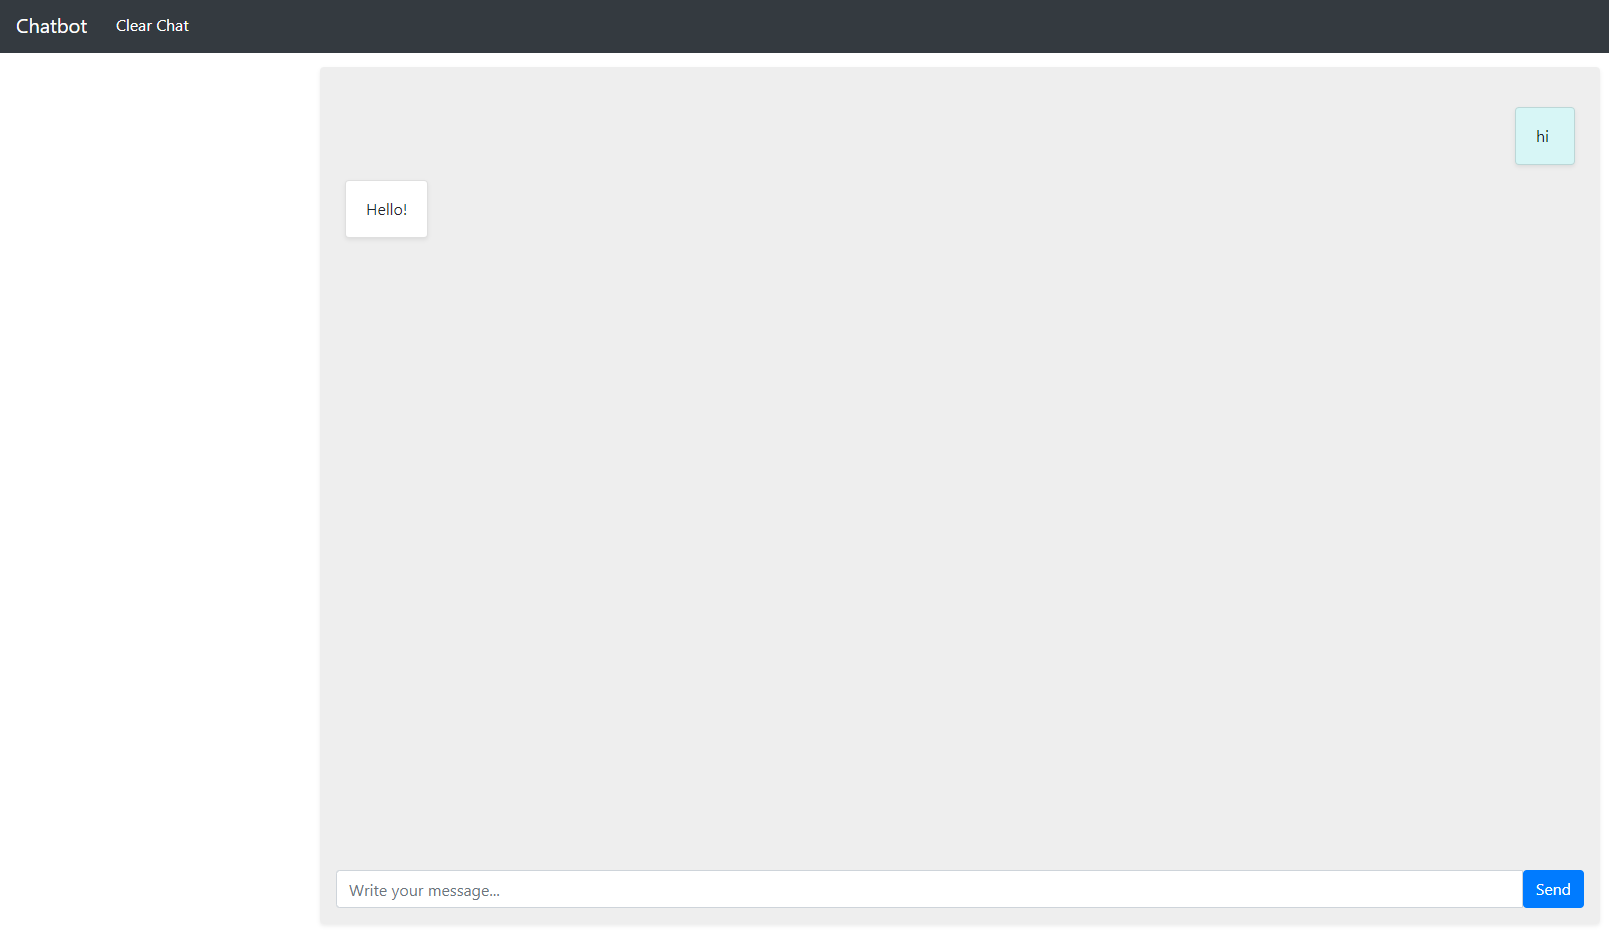
\includegraphics[width=8cm, valign=m]{tests/f1} & Yes \\
		\midrule
		F3 & User Input
		& The user should be enter queries to the bot using a textbox input
		& 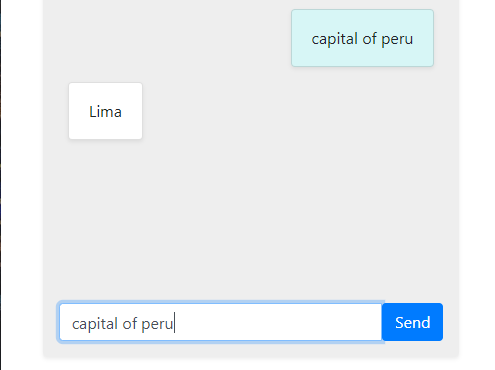
\includegraphics[width=8cm, valign=m]{tests/f3} & Yes \\
		\midrule
		F4 & Responses on Page
		& The should see the chatbot response on the web page
		& 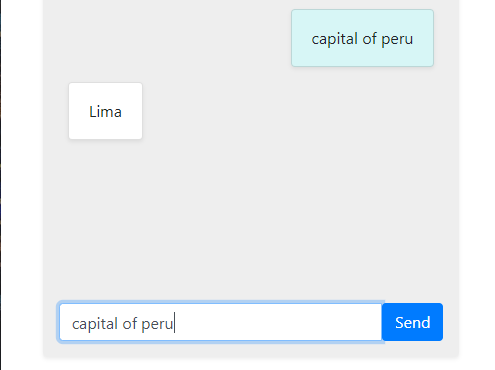
\includegraphics[width=8cm, valign=m]{tests/f3} & Yes \\
		\midrule
		F5 & Conversation History
		& The should see the whole conversation with the bot on the page
		& 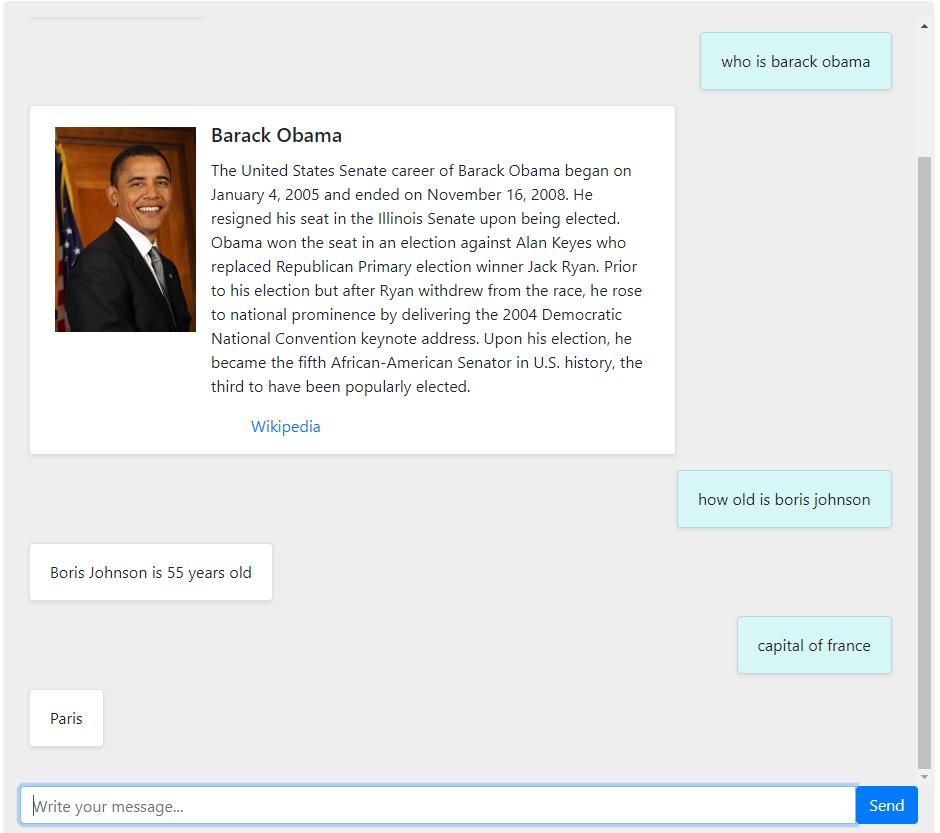
\includegraphics[width=8cm, valign=m]{tests/f5} & Yes \\
		\midrule
		F6 & Person Description Query
		& The user should be able to ask a query about who a person is\newline - 'WHO IS *' and receive a description of that person
		& 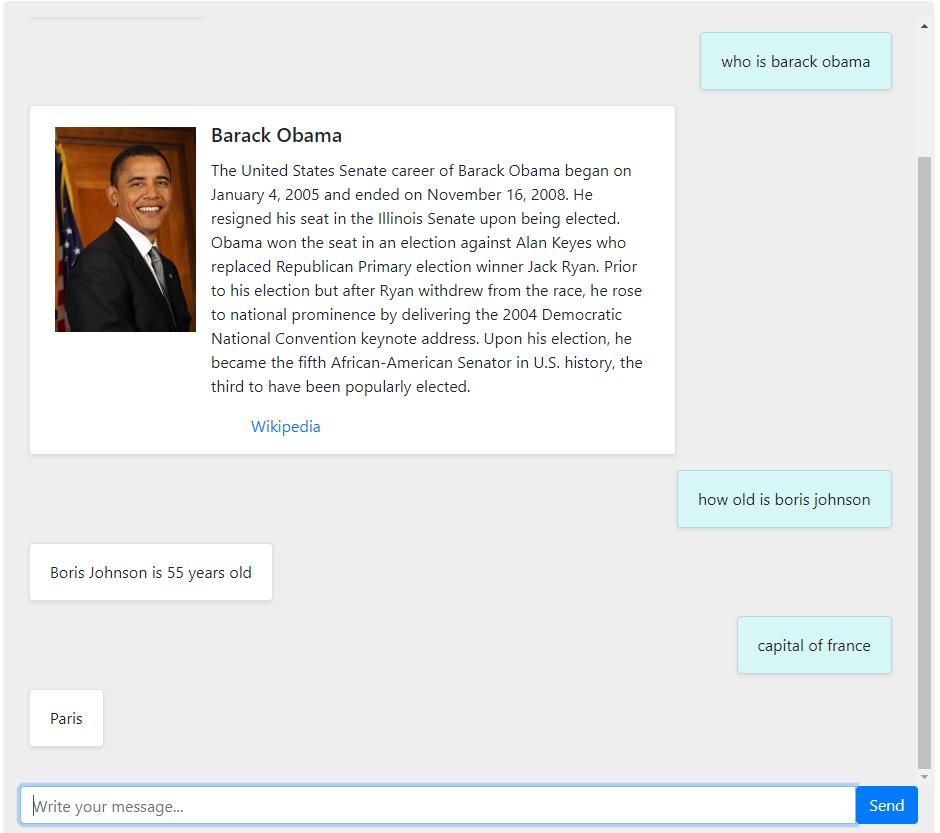
\includegraphics[width=8cm, valign=m]{tests/f5} & Yes \\
		\midrule
		F7 & Person Birthdate Query
		& The user should be able to ask a query about when a person was born\newline - 'WHEN WAS * BORN' and see their birth date
		& 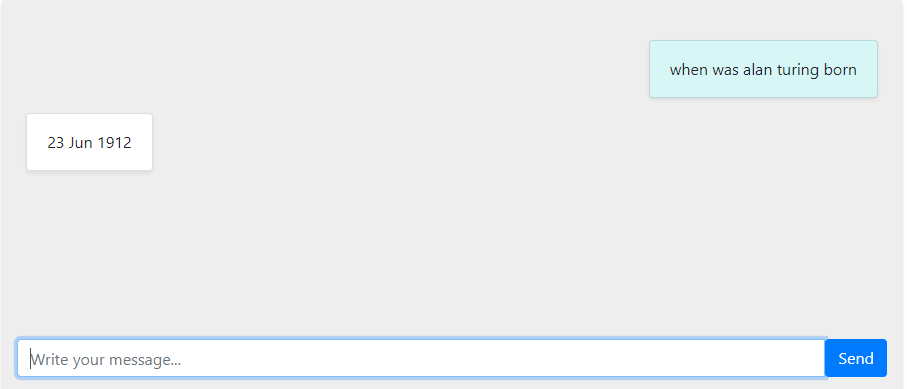
\includegraphics[width=8cm, valign=m]{tests/f7} & Yes \\
		\midrule
		F8 & Person Age Query
		& The user should be able to ask a query about a person's age\newline - 'HOW OLD IS *' and see their age
		& 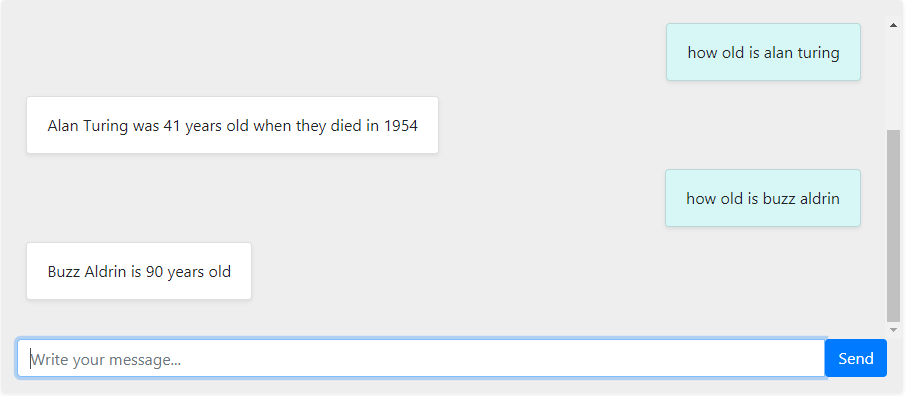
\includegraphics[width=8cm, valign=m]{tests/f8} & Yes \\
		\midrule
		F9 & Person Birthplace Query
		& The user should be able to ask a query about where a person was born\newline - 'WHEN WAS * BORN' and see their birthplace
		& 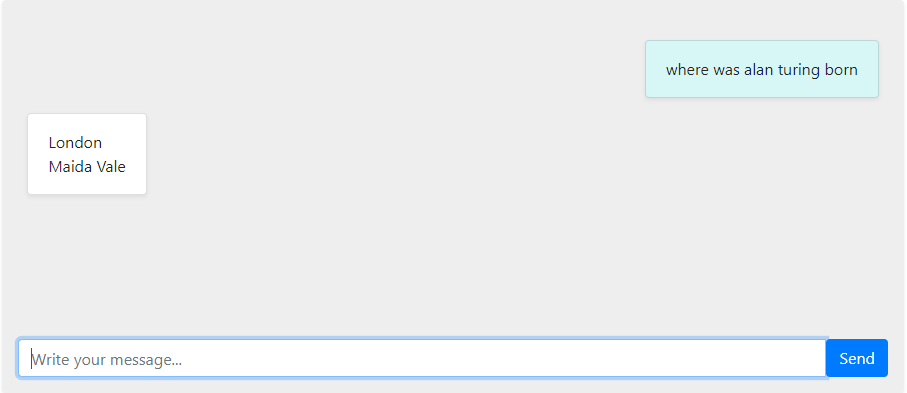
\includegraphics[width=8cm, valign=m]{tests/f9} & Yes \\
		\midrule
		F10 & Person Death Date query
		& The user should be able to ask a query about when a person died\newline - 'WHEN DID * DIE' and see their death date
		& 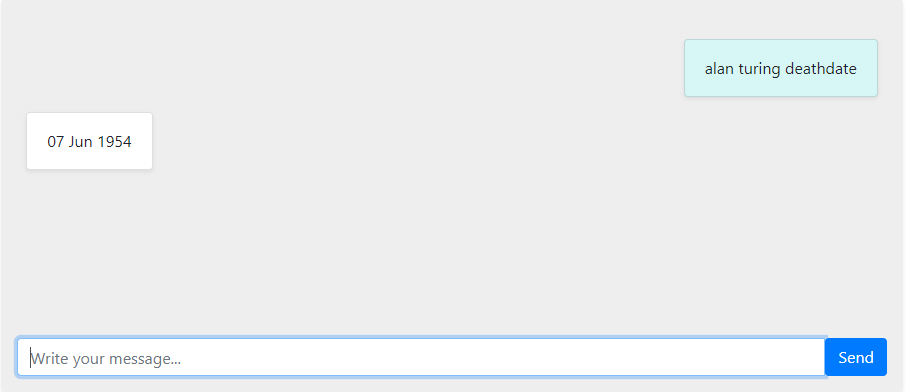
\includegraphics[width=8cm, valign=m]{tests/f10} & Yes \\
		\midrule
		F11 & Person Known For Query
		& The user should be able to ask a query about what a person is known for\newline - 'WHAT IS * KNOWN FOR' and see what they are known for
		& 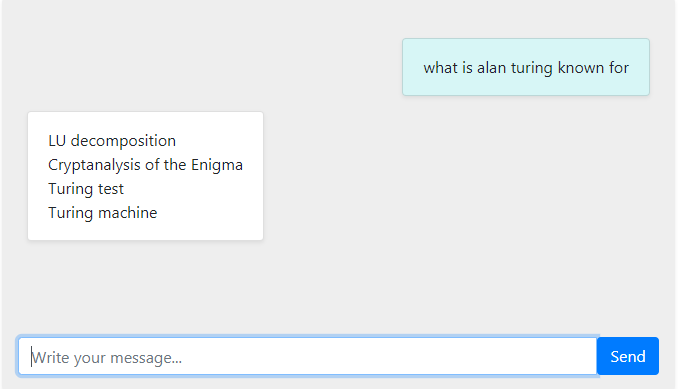
\includegraphics[width=8cm, valign=m]{tests/f11} & Yes \\
		\midrule
		F12 & Person Photo Query
		& The user should be able to ask for a photo of a person\newline - 'WHAT DOES * LOOK LIKE' and see a photo of the person
		& 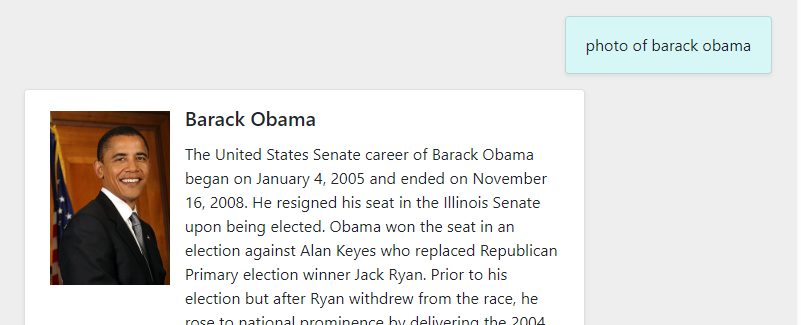
\includegraphics[width=8cm, valign=m]{tests/f12} & Partial\footnote{\label{fn:discuss}Discussed in Section~\ref{subsec:requirementresults}} \\
		\midrule
		F13 & Person Wikipedia Link Query
		& The user should be able to ask for the link to a person's Wikipedia page\newline - '* WIKIPEDIA PAGE' and receive a link to their page
		& 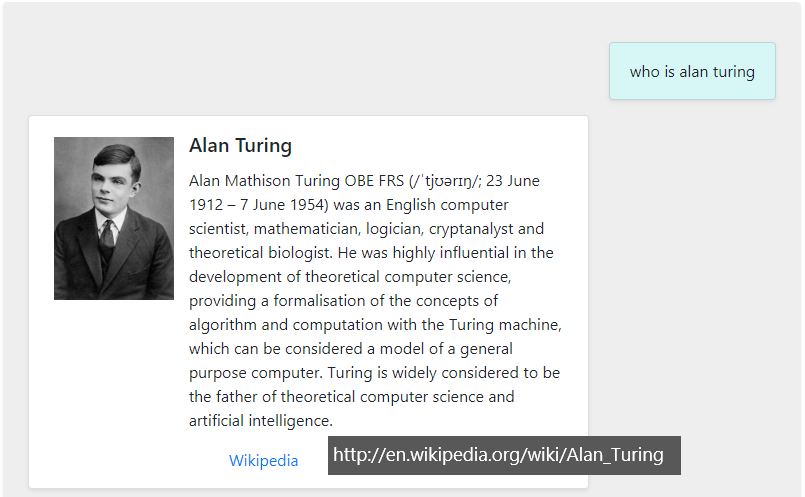
\includegraphics[width=8cm, valign=m]{tests/f13} & Yes \\
		\midrule
		F14 & Country Description Query
		& The user should be able to ask about a country\newline - '[COUNTRY]' and see a description of that country
		& 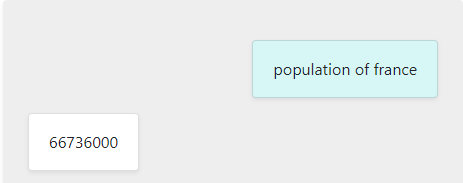
\includegraphics[width=8cm, valign=m]{tests/f14} & Yes \\
		\midrule
		F15 & Country Population Query
		& The user should be able to ask about a country\newline - '[COUNTRY] POPULATION' and see the population of that country
		& 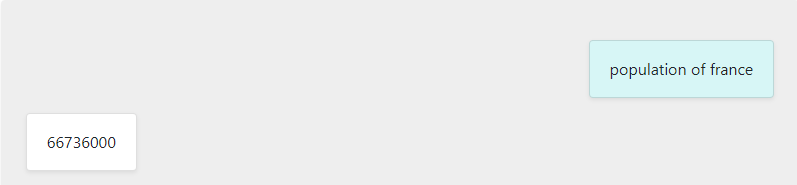
\includegraphics[width=8cm, valign=m]{tests/f15} & Yes \\
		\midrule
		F16 & Country Capital Query
		& The user should be able to ask for the capital of a country\newline - 'CAPITAL OF [COUNTRY]' and see the capital of that country
		& 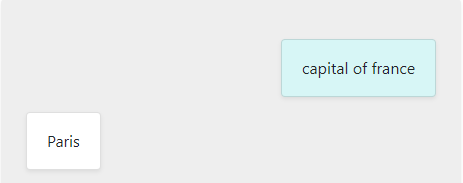
\includegraphics[width=8cm, valign=m]{tests/f16} & Yes \\
		\midrule
		F17 & Person List Query
		& The user should be able to ask for lists of people\newline - 'LIST OF ACTORS' - and see a list of actors 
		& 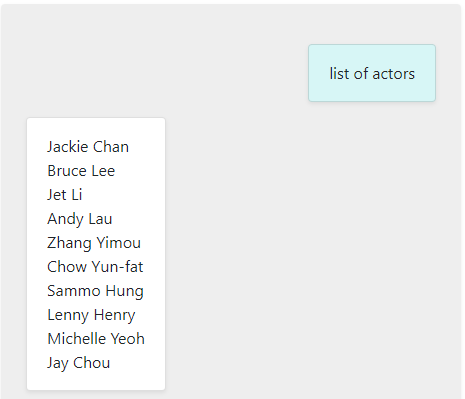
\includegraphics[width=8cm, valign=m]{tests/f17} & Yes \\
		\midrule
		F18 & Person AND Query
		& The user should be able to combine queries\newline - 'LIST OF ACTORS BORN IN 1980 AND BORN IN LONDON'\newline and see a list matching that conditional query
		& 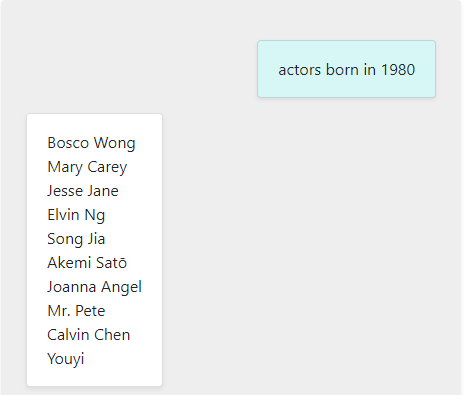
\includegraphics[width=7cm, valign=m]{tests/f18} & Partial \textsuperscript{\ref{fn:discuss}} \\
		\midrule
		F19 & Context-aware Conversation
		& The user should be able to continue from previous queries using pronouns\newline e.g. 'WHEN WAS HE BORN' and the chatbot should maintain the context of the query
		& 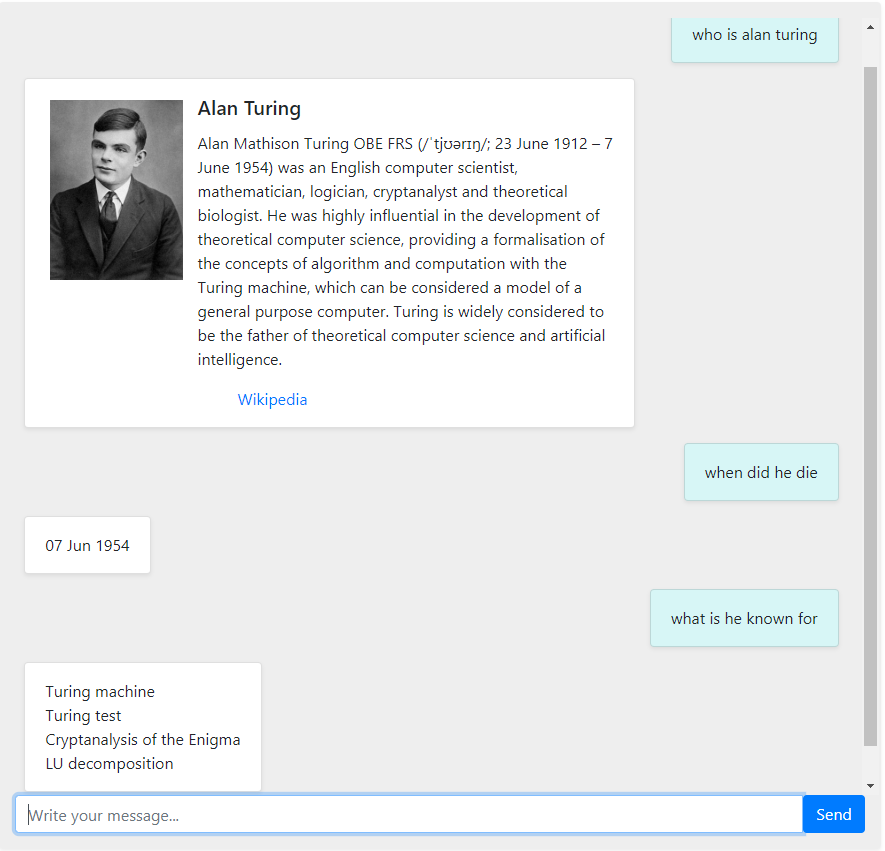
\includegraphics[width=8cm, valign=m]{tests/f19} & Yes \\
		\midrule
		F20 & Chatbot Greeting
		& The chatbot should be able to greet the user
		& 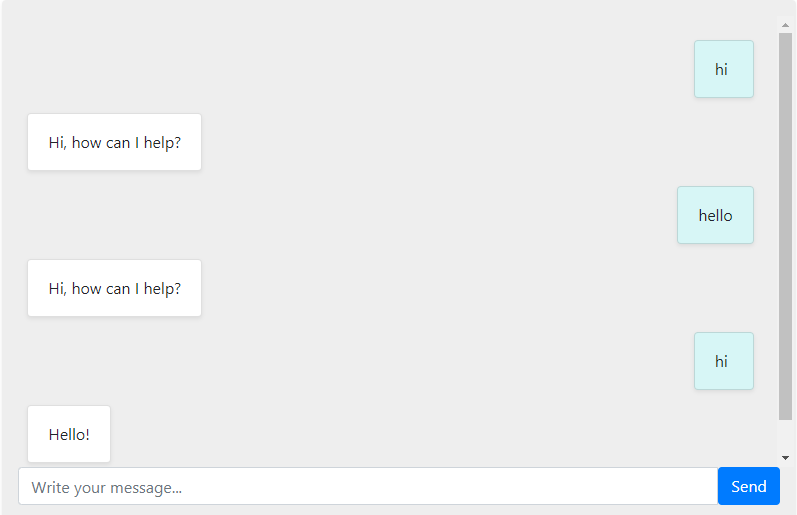
\includegraphics[width=8cm, valign=m]{tests/f20} & Yes \\
		\midrule
		F21 & Chatbot Examples
		& The chatbot should display a list of example queries\newline when asked 'EXAMPLES' or 'WHAT CAN YOU DO'
		& 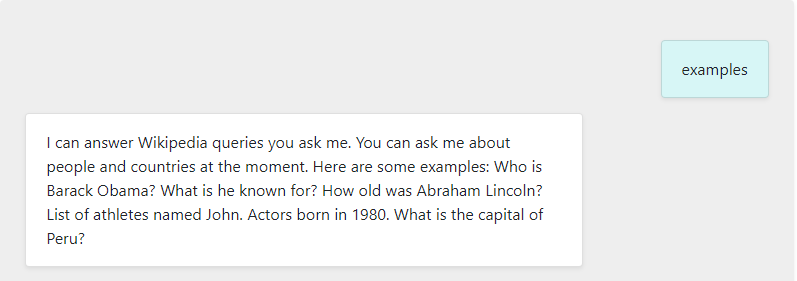
\includegraphics[width=8cm, valign=m]{tests/f21} & Yes \\
		\midrule
		F22 & Chatbot Help
		& The user should be able to receive help from the chatbot\newline on how to use it when asked 'HELP'
		& 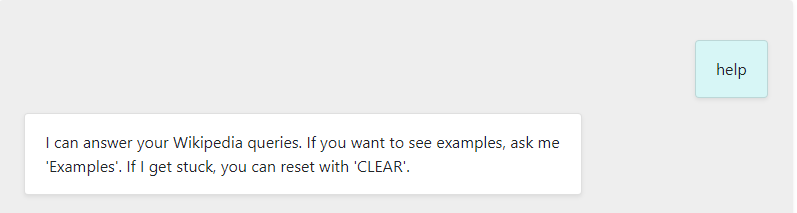
\includegraphics[width=8cm, valign=m]{tests/f22} & Yes \\
		\bottomrule
		\caption{Requirements testing and evidence}
		\label{tab:testreq}
	\end{tabularx}
\end{landscape}

\newpage
\subsection{Performance Testing}
\begin{itemize}
	\item P1: Web page loads in 5 seconds
	\item P2: Chatbot response in 5 seconds
	\item P3: Application functions without failure
	\item P4: Any errors are logged and the user is informed of an error
\end{itemize}

\subsection{Results}
\label{subsec:requirementresults}

\section{Unit Testing}

\section{User Acceptance Testing}
Although we have tested the requirements specification, it is important that we assess the accuracy and ability of the system as a whole. For example, we may get a response from the system, but it may not be the result we were expecting. As such, the three testers will be given access to the system in order to answer many unseen questions and assess their output.

In order to formalise this, the users were asked to document the exact query they entered, the result they received, and whether or not it was the result they were expecting, in line with the questions in the specification. They were also asked to ask it further questions beyond the scope of the specification, so that we can establish logical future developments for the system. The format of their testing results is as follows:
\begin{itemize}
	\item Test Number
	\item Requirement (F\#)
	\item Input
	\item Output
	\item Result as expected?
	\item Comments
\end{itemize}
They were asked to test at least 5 queries for each requirement item, followed by at least 10 queries not related to the requirements, and document their results with comments. For anonymity, each user's results are shown in Figures~ with a user number.

\section{Conclusion}